\documentclass[ngerman, 12pt, pdftex]{scrartcl}[2006/07/30]

%encoding and input
\usepackage[ngerman]{babel} %spell correction
\usepackage[utf8]{inputenc} 
\usepackage[T1]{fontenc}

%bugfixes
\usepackage{fixltx2e} 

%Font Symbols and Colors
\usepackage{textcomp} %more symbols
\usepackage{xcolor}
\usepackage{hyperref}

%Math
\usepackage{amsmath}
\usepackage{mathtools} %extends amsmath

%Programming
\usepackage{listingsutf8} %in utf8
\lstset{language=Java,captionpos=b,tabsize=3,frame=,keywordstyle=\color{blue},commentstyle=\color{teal},stringstyle=\color{red},numbers=none,numberstyle=\tiny,numbersep=5pt,breaklines=false,showstringspaces=false,basicstyle=\footnotesize,emph={label},upquote=false} %Syntax highlighting

%Verbatim extension (with line numbers and tab-expansion)
\usepackage{moreverb} 

%Headers and Footer
\usepackage{fancyhdr}

%title
\title{Dokumentation}
\author{Frank M\"{u}ller, Oliver Wisler, Lucius Bachmann, Fabio Sulser}
\subtitle{Swissdefcon-Team}

\begin{document}
%declare  Header
\pagestyle{fancy}
\fancyhf{} 
\fancyhead[L]{Dokumentation} %left header
\fancyhead[C]{Swissdefcon-Team} %centered header
\fancyhead[R]{\thepage}  % right header
\renewcommand{\headrulewidth}{0.1pt} 	%upper separating line
%\fancyfoot[C]{\thepage} 				%centered footer, line number



%you might want to enable come features:
\maketitle
%\listoffigures 
%\listoftables


\newpage

\tableofcontents

\newpage

\section{Grobaufbau}
Unser Projekt gliedert sich in 5 grosse Pakete, alle Klassen welche Client und Server übergreifend verwendet werden, 
befinden sich im Paket "shared". Der ganze Server befindet sich im Paket "server" und der Client im Paket "Client".
Zum Ausprobieren und testen während dem Programmieren, als auch für den Unittest gibt es das Paket "test".

%-- Client
\section{Client}
\subsection{Aufbau}
Der Client gliedert sich in 6 Pakete, wovon 4 der Datenverwaltung dienen und 2 jeweils für die Lobby oder das Spiel zuständig sind.
Eine kurze Beschreibung der Pakete findet sich in der folgenden Tabelle:
\begin{table}[h!]
\begin{tabular}{ l p{12cm} }
  Paketname & Zweck \\ \hline
  net &  stellt Klassen für die Kommunikation und Serversuche zur Verfügung. In diesem Paket werden alle empfangenen Daten ausgewertet und mittels Event oder statischen Funktionen weitergeleitet.\\
  events & Stellt Events zur Verfügung welche für die interne Kommunikation im Client genutzt werden. (GameEvent, ChatEvent)\\
  data&  haltet Daten welche für das Spiel oder die Lobby wichtig sind (die Spielerid, Zuordnung Spieler zu Id, etc...).\\
  resources & Stellt eine Klasse zur Verfügung mittels derer Daten (Bilder, etc...) geladen werden können.\\
  lobby & Beinhaltet die ganze Lobby\\
  game & Beinhaltet das GUI für das Spiel\\
\end{tabular}
\caption{Unterpakete im Paket client}
\end{table}
\begin{figure}[h!]
\centering
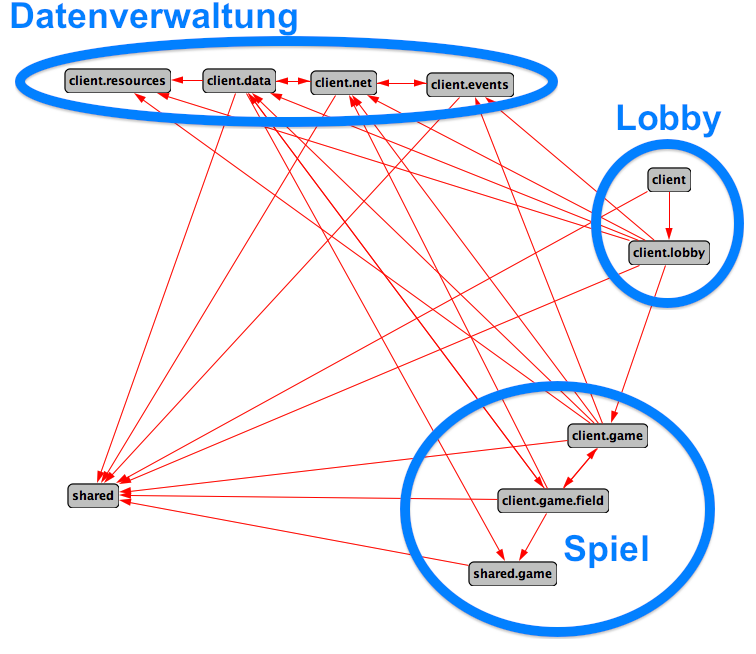
\includegraphics[scale=0.4]{client/client_aufbau_ann.png}
\caption{Importe zwischen den Paketen}
\end{figure}

\subsection{Datenverwaltung}
Ausgehend vom Parser werden die Daten mit zwei Methoden verteilt.
Daten welche nicht permanent gespeichert werden müssen (z.Bsp. Chatnachrichten) werden per Event 
weitergeleitet, so dass von überall her mit einem geeigneten Listener darauf zugegriffen werden kann.
Daten welche langfristig gespeichert werden (zum Beispiel die Zuordnung von Spielernamen zu ihrer Id) werden
von Klassen im Paket "client.data" gespeichert. Darunter fällt  "PlayerManager" welcher alle Informationen bezüglich Spieler speichert und "RunningGame" welche alle Informationen zum gerade laufenden Spiel bereithält.
Auf diese gespeicherten Daten kann mittels statischer Methoden jederzeit vom Spiel oder von der Lobby zugegriffen werden.

\begin{figure}[h!]
\centering
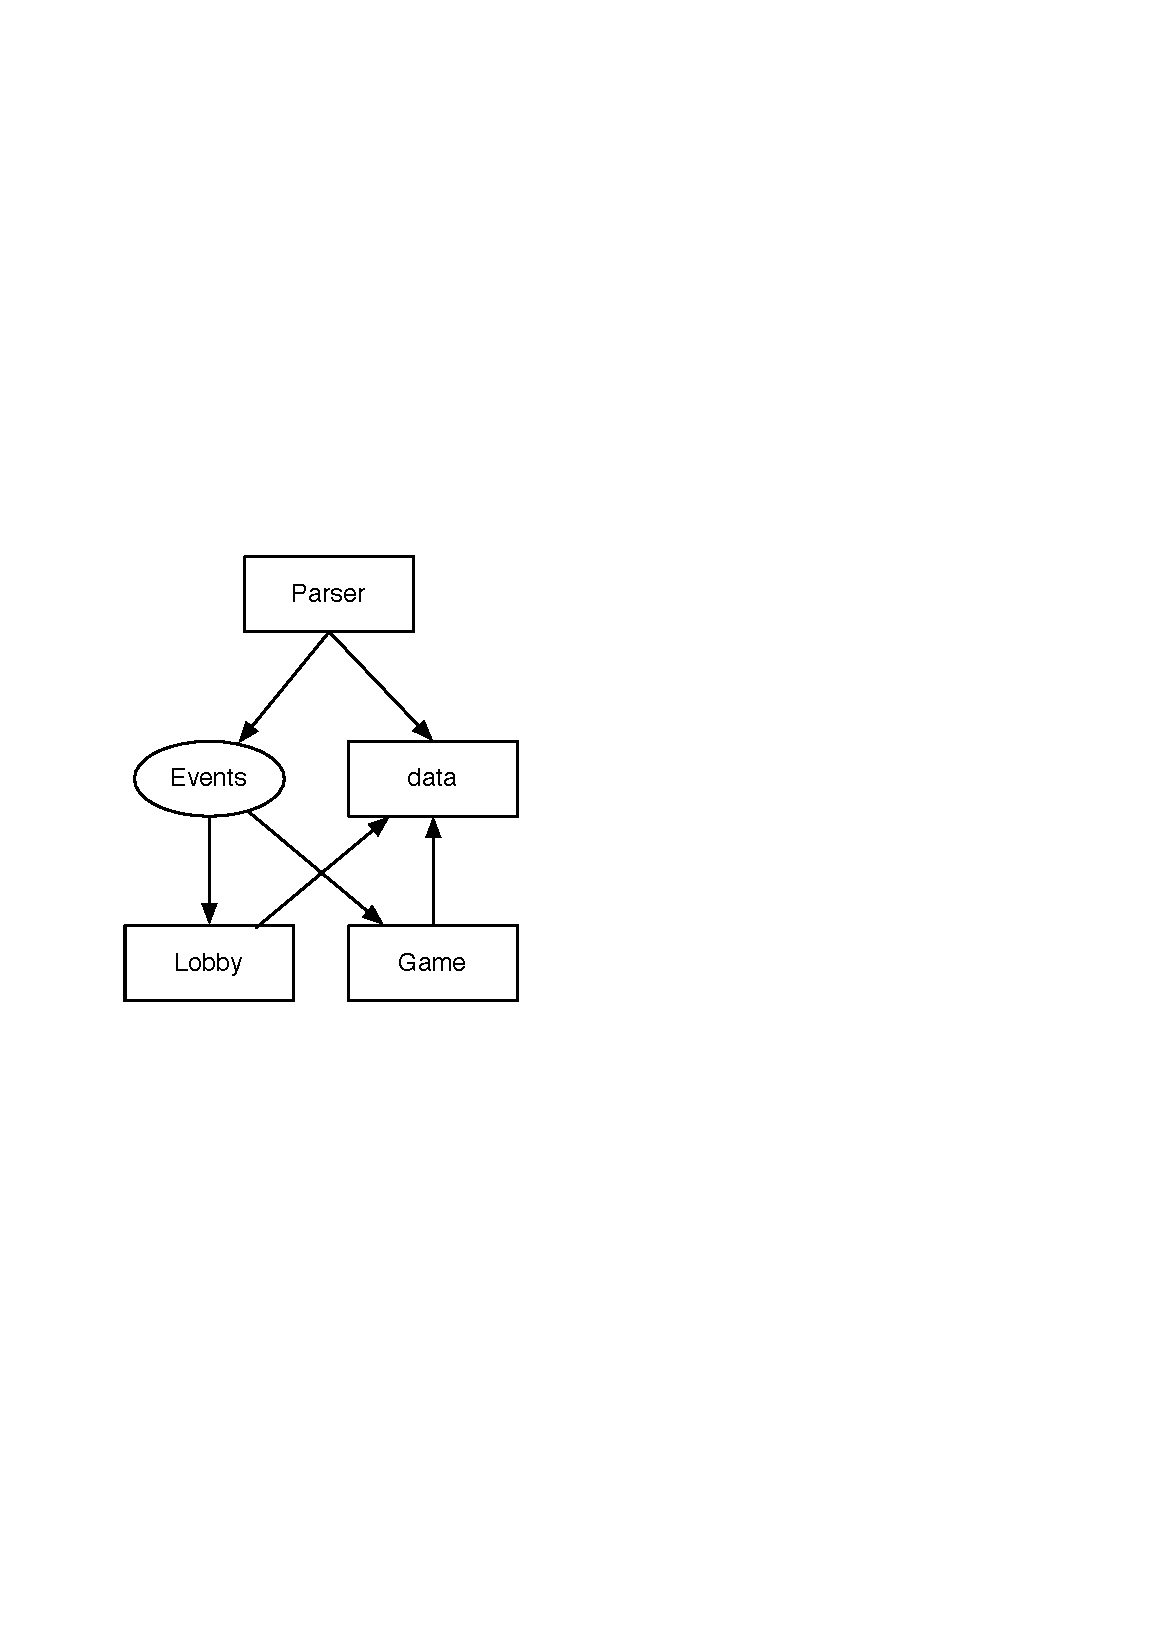
\includegraphics[scale=0.6]{client/datenhaltung.pdf}
\caption{Datenverteilung}
\end{figure}

\subsection{Rendering}

%todo fabio

%-- Server
\section{Server}

%todo frank

\subsection{Aufbau}
\subsection{Datenverwaltung}

%todo frank und lucius

\subsection{Spiellogik}
\subsection{Aufbauphase}
Mit dem Start des Spiels wird der GamePlayObjectManager instanziert. Er verwaltet die GamePlayObjects.
Wird ein Objekt erstellt, \"{u}bergibt man dem Objekt den GamePlayObjectManager. Das Objekt, falls es an einer g\"{u}ltigen Position gesetzt wurde und der Spieler noch Geld hat, tr\"{a}gt sich dann in die Liste AllObjects und, wenn ein Defensivobjekt, in die Liste Defensives ein. Wird ein Objekt bewegt, dann wird das in die Membervariable Target eingetragen.

\subsection{Runde}

Wird jetzt die Runde gestartet, dann..
\begin{itemize}

\item Testet der GamePlayObjectManager zuerst, ob ein Spieler noch Population hat. Wenn nicht, werden all seine Objekte gel\ "{o}scht und sein Geld auf 0 gesetzt.
\item Darauf werden die Objekte gepr\"{u}ft, ob sie noch Lebenspunkte haben. Wenn nicht, werden sie gel\"{o}scht.
\item Dann rechnet jedes Objekt aus, wohin es sich bewegen wird. Falls ein Objekt weiter als seine MovingRange bewegt werden sollte, dann bewegt es sich in Richtung Target soweit, wie es die MovingRange erlaubt. Das Ergebnis wird in moveProv gespeichert.
\item Jetzt senden alle Objekte allen Objekten ihre Bewegung, und jedes Objekt testet die eingegangenen Bewegungen darauf, ob sie durch ihren Angriffsradius verlaufen. Wenn ja und angreifbar, werden sie in der Liste possibleTargets gespeichert. Dann werden die Objekte auf ihre neue Position gesetzt.
\item Schiesslich f\"{u}hren alle Objekte ihre Angriffe aus. Die Banken geben Geld, die Reproduktionszentren Geld. Alle anderen Objekte w\"{a}hlen zuf\"{u}llig ein Objekt aus den possibleTargets aus, schiessen darauf bis es keine Lebenspunkte mehr hat, wenn es 0 Lebenspunkte hat w\"{a}hlen sie das n\"{a}chste Objekt, bis sie keine Munition mehr haben.
\end{itemize}



%-- Kommunikation
\section{Kommunikation}
\subsection{Serverauswahl}

%todo frank

\subsection{Verbindung}

%Todo frank

\subsection{Protokoll}
\subsubsection{Aufbau}
Jeder Protokolbefehl besteht aus 5 Buchstaben. Der erste Buchstaben bezeichnet jeweils den Bereich des Befehls, es sind dies:
\begin{itemize}
\item D für die Serversuche
\item V für Befehle betreffend der Verbindung
\item C für den Chat
\item G für das Spiel
\end{itemize}
\subsubsection{Befehle}
Alle Protokolbefehle können im Wiki unter \url{http://chaos-theory.ch/CS108/wiki/doku.php?id=protocol} abgerufen werden.

\section{Andere Pakete}
\subsection{shared}
Hier sind diverse Klassen, welche sowohl vom Server als auch vom Client benutzt werden.
Darunter fällt das Protokoll, ein InputValidator, welcher Eingaben validieren kann, Eine Klasse welche Log Funktionen zur Verfügung stellt,
diverse Einstellungen (Spiel und Kommunikation).

%-- Unittest
\section{Unittest}

%TODO lucius

\end{document}